\chapter{Overall Description}

\section{Product perspective}
In this section we analyze a list of real 
scenarios and diagrams illustrating further details about shared phenomena.

\subsection{Scenarios}
\begin{enumerate}
    \item \textbf{Registration} \\
    Prof. White reads about CodeKataBattle in a online spot and decides to use the platform to 
    challenge his students. So, he creates an account using his email address and personal information 
    and convinces his colleagues to join the platform.\\
    Alice and her classmates, after prof. White's lesson, are interested in improving their coding 
    skills and sign up to CKB. Alice provides her email address and personal information; after the email 
    confimation goes well, 
    she can complete the registration process by linking her CKB account to her GitHub account.\\
    After the registration, both Prof. White and Alice can visualize the profile of all the other 
    students and the information about the ongoing tournaments.

    \item \textbf{Creation of tournaments} \\
    Prof. Brown and Prof. Smith want to decide whose class is better at programming. So Prof. Brown 
    creates a tournament on CKB and invites his colleague to create battles within the tournament. Prof. Brown 
    sets a deadline by which their students can subscribe. A notification is sent to all CKB students.
    
    \item \textbf{Creation of battles} \\
    Prof. Bloom has been granted the permission to create battles in a tournament, so he uploads a 
    code kata. First he writes a brief textual description of the exercise, then he includes 
    the software project with build automation scripts and test cases. He also sets some rules: 
    minimum and maximum number of students per group, registration deadline, final submission deadline, and
    automated evaluation parameters.\\
    Finally, he chooses to include an optional manual evaluation of his students' work.

    \item \textbf{Students join a battle} \\
    Bob registered to the CKB platform and received a notification about an interesting tournament 
    and he subscribed to it. \\
    He is notified about a new interesting upcoming battle in that tournament. Before the registration 
    deadline expires, Bob can form a group, so invites his girlfriend Eva to join him. After the registration 
    deadline ends, they are sent the link of the GitHub repository of the code kata. To be able to start 
    working on the project, Bob and Eva must fork the repository and set up an automated workflow through 
    GitHub Actions to inform the CKB platform about their commits.

    \item \textbf{Upload of a solution} \\
    Charlie has joined a battle with his friends and thinks that they have found a good solution to 
    the assigned problem. So he pushes his code before the final deadline to the main branch of their 
    repository. \\This battle does not expect any manual evaluation by the educator, so as soon as 
    they push the solution, the platform evaluates it and they can visualize their updated battle score. 
    After the final deadline has expired, Charlie can also see the current tournament rank. 

    \item \textbf{Evaluation of a project}\\
    When Prof. Cooper created the battle, he decided to include manual evaluation in the battle rules: 
    he wants the system to assign up to 75 points, while he will assign the remaining 25 points. 
    So, scores will always be between 0 and 100.\\
    After the final deadline, prof. Cooper can see all the groups' work and he evaluates them according 
    to some personal parameters such that design quality, code cleanliness, compliance with specifications.

    \item \textbf{Creation of gamification badges}\\
    Prof. Moore has created a tournament and to spice things up he decides to include badges. 
    These are awarded according to the rules specified by him at tournament set up time: in particular, 
    he wants to reward the student with most commits and the student who have attended the most battles.\\
    The badges are assigned at the end of the tournament and the collected badges can be seen by everyone 
    visiting the student's profile. \\
\end{enumerate}

\subsection{Class diagrams}
The UML class diagram below represents a conceptual, high-level model of the system to be. 
At this level, it does not include any references to methods and other low-level details, those will be detailed during the design phase. \\

\begin{figure}[H]
      \centering
      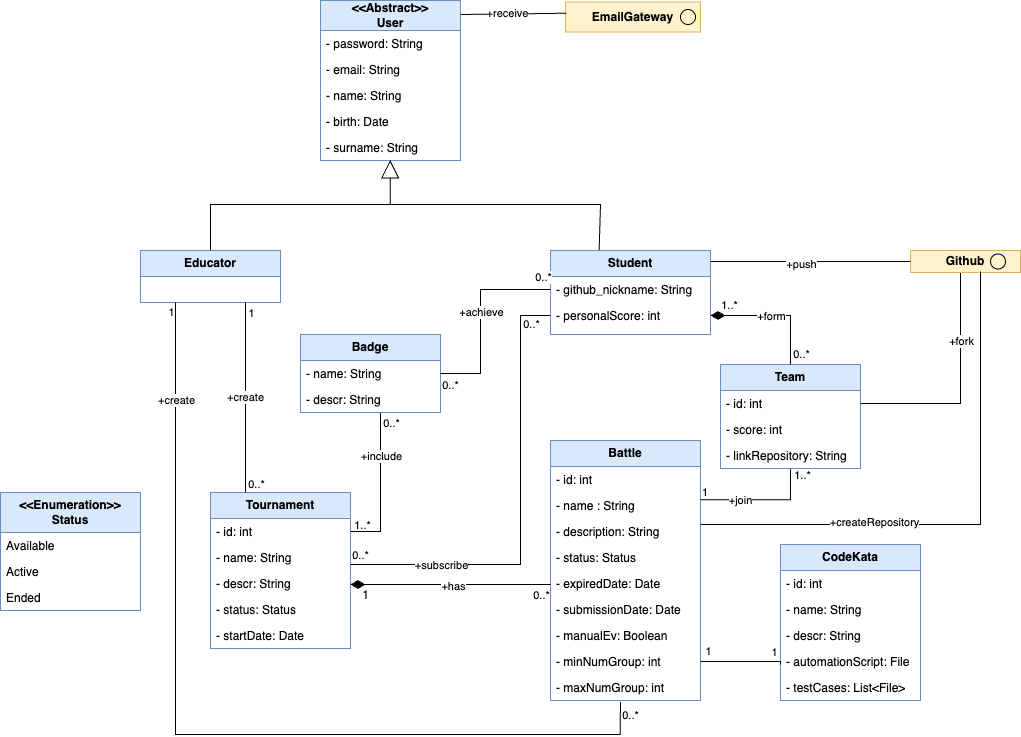
\includegraphics[width=1\textwidth]{images/Class_Diagram.png}
      \caption{Class diagram}
\end{figure}

The main entities in the diagram are:
\begin{itemize}
    \item \textbf{User:} represents an user of the system who can access to the platform with his credentials.
    \item \textbf{Student:} represents a student, a particular type of user who can join tournaments and battles.
    \item \textbf{Educator:} represents an educator, a particular type of user who can create tournaments, battles and badges.
    \item \textbf{Tournament:} represents a tournament, a programming competition composed of various battles created by an educator.
    \item \textbf{Battle:} represents a battle with a specific code kata created by an educator, in which teams of students can compete.
    \item \textbf{Team: } represents a group of students who can compete in a battle.
    \item \textbf{Badge: } represents an award that educator can create for a tournament and assign to eligible students.
    \item \textbf{CokeKata: } represents a programming exercise in a programming language chosen by its creator. 
    It includes automation scripts and test cases.
\end{itemize}

\subsection{State diagrams}
State diagrams model the behavior of a single object and are used for objects with 
significant dynamic behavior; they also specify the sequence of states that an 
object goes through during its lifetime in response to stimuli from the environment.
In particular, they show the life history of a given class, the events that cause a transition
from one state to another and the actions that result from a state change.\\
In this section we will represent the main state diagrams of the whole system.

\textbf{Tournament}\\
In the following figure the possible status of a tournament is shown. \\
\begin{figure} [H]
  \centering
  \includegraphics[width=0.815\textwidth]{images/state_diagrams/Tournament.png}
  \caption{Tournament state diagram}
\end{figure} \vspace{1cm}

\textbf{Battle}\\
In the following figure the possible status of a battle is shown. \\
\begin{figure} [H]
  \centering
  \includegraphics[width=0.815\textwidth]{images/state_diagrams/Battle.png}
  \caption{Battle state diagram}
\end{figure} \vspace{1cm}


\section{Product functions}
\subsection{Sign up and login}
These functions are available to both students and educators.\\
The sign up functionality allows users to register on the platform: in particular, each user will provide an email 
and a password. Also, the user must provide their personal information (name, surname, date of birth) and 
if the user is a student they are required to provide a GitHub account.\\
Then a verification email is sent to the user.
Once registered, both students and educators can visualize the profile of all the other students.\\
The login functionality allows users to access the platform using their email and password.\\

\subsection{Creation of a tournament}
Educators can create tournaments, programming competitions composed of various code kata battles.\\
The creator of the tournament can invite other educators and grant them the permission to create battles within the 
context of the tournament.\\
When they create a tournament, educators set a registration deadline and can also define badges, i.e., awards that 
represent particular achievements of individual students: the educator may use pre-defined variables and rules or create 
new ones. Badges are awarded automatically at the end of a tournament.\\
Information about ongoing tournaments is availaible to all subscribed users.\\

\subsection{Creation of a battle}
After being granted such permission from the creator of the tournament, educators can create code kata battles within the
context of the tournament.\\
To create a battle, the educator must upload the code kata, set the rules regarding groups composition (minimum and maximum 
number of members), set a registration deadline, set a final submission deadline, and set evaluation parameters. They may also 
specify if they want to include a manual evaluation of the students' work, in addition the mandatory automated one, after the 
submission deadline expires.\\
Users can see the current battle rank evolving during the battle.\\

\subsection{Joining a tournament}
Students can join any tournament before its registration deadline expires. By signing up to a tournament, they also 
subscribe to notifications regarding upcoming battles within the context of that tournament.\\
Students also receive a notification when the tournament ends.\\
By participating in a tournament, students can earn badges that can be visualized in their profile.\\

\subsection{Joining a battle}
Students subscribed to a tournament can join any upcoming battle before its registration deadline expires.\\
Students can participate alone or in groups to the battle, according to the rules set for that battle by its creator.\\
When the registration deadline expires, students are sent an email with the link of the GitHub repository containing the 
code kata. To start working on the project, they are required to fork the repository and set up an automated workflow, 
using GitHub Actions, to inform CKB about new commits into the main branch of their repository.\\
As soon as students push a solution it is automatically evaluated, so they can see their current battle score and their 
battle ranking.\\
When the submission deadline (and, if required, the manual evaluation stage) ends, students are notified about their final 
battle score and ranking and they can see their updated tournament score.\\

\subsection{Evaluation of a project}
According to the parameters set by the creator of the battle, the system automatically evaluates the students' work with regard to
\begin{enumerate}
  \item functional aspects (i.e., the percentage of passed test cases);
  \item timeliness (i.e., the time passed between the registration deadline and the last commit);
  \item code quality (extracted using static analysis tools).
\end{enumerate}
If the educator has decided to include manual evaluation in the battle rules, they can see all the groups' work and evaluate 
the students' work according to some personal parameters such as design quality, code cleanliness, compliance with specifications.\\
The final score is a natural number between 0 and 100 calculated as specified at battle creation time.\\

\section{User characteristics}
The CKB system has two different types of actors who use the system:
\begin{itemize}
    \item \textbf{Educator:} people who create tournaments and battles, and evaluate the students' work. 
    To create a battle they set up some settings such as the code kata (description and software project, including test cases and build
    automation scripts), the minimum and maximum number of students per group, the registration deadline, the final submission deadline, and the configurations for scoring.
    They can also grant other educators the permission to create battles within a tournament. 
    For each tournament, they may define specific badges establishing new rules and variables in order to reward capable students.
    Optionally, they can manually evaluate students' code based on their requirements and assign their personal score. 
    \item \textbf{Student:} people who join tournaments and battles created by educators, and commit their code on GitHub. 
    They can create a team inviting other students and compete in a battle with other teams. 
    At the end of each tournament they can visualize the final rank and their current score. 
    If educators has defined some specific badges for the tournament, students can achieve them if they have fulfilled the rules. 
    They can visualize the achieved badges on their personal profile. 
\end{itemize}

\section{Assumptions, dependencies and constraints}

\subsection{Domain assumptions}
\begin{table}[H]
  \begin{tabularx}{\textwidth}{cX}
        \toprule
        \textbf{D1} & Users provide correct information during the registration process.\\
        \textbf{D2} & Students have an email and a GitHub account.\\
        \textbf{D3} & Users have a stable and reliable Internet connection.\\
        \textbf{D4} & Students know the functioning of GitHub and GitHub Actions.\\
        \textbf{D5} & Educators create at least one battle within a tournament.\\
        \textbf{D6} & Students must give consent to access their GitHub account.\\
        \textbf{D7} & Educators have a good knowledge of programming.\\
        \textbf{D8} & Educators upload a correct code kata.\\
        \bottomrule
  \end{tabularx}
\end{table}

\subsection{Dependencies}
\begin{table}[H]
      \begin{tabularx}{\textwidth}{cX}
            \toprule
            \textbf{Dep1}  & The system requires access to GitHub API.\\
            \textbf{Dep2}  & The system will use a third party API to send emails to the users.\\
            \textbf{Dep3}  & The system will require internet connection to interact with all the users.\\
            \textbf{Dep4}  & The system requires access to a development environment to run students' code.\\
            \bottomrule
      \end{tabularx}
\end{table}

\subsection{Constraints}
\begin{itemize}
      \item The system shall be compliant to local laws and regulations, in particular users data should be treated
            according to the GDPR. This means that users should be always able to request their data.
      \item The system should collect only necessary data, such as name, surname, date of birth, email address, etc.
      \item To better protect the users' sensitive information, such as their personal information and credentials, their data 
            should be encrypted.
      \item The external APIs, especially those critical for the correct functioning of the system, must be chosen among those with 
            the highest availability and reliability.
\end{itemize}
